%\section{Introduction}
%In the late 1800s Svante Arrhenius and Jacobus Henricus van't Hoff observed that reaction rates, $k$, are on the form of
%\beq{arrhenius}
%k = A e^{E_a/\kB T},
%\eeq
%where $E_a$ is an activation energy with a prefactor $A$.~\cite{vant-hoff-1884, arrhenius-1889}
%\expand

\section{Motivation}
\subsection{The Time-scale Problem}
\label{sec:tst-timescale-problem}

\begin{figure}[h]
\begin{center}
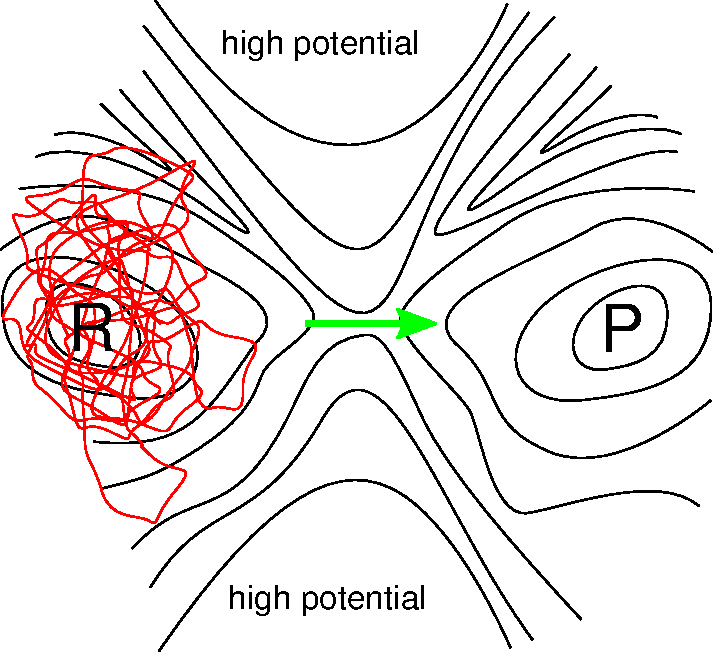
\includegraphics[width=0.5\linewidth]{timescale-problem}
    \parbox{0.85\linewidth}{
\caption{The time-scale problem.
The system will mostly spend time near the minimum of the reactants basin (R), the red trajectory, while the reactions of interest, green arrow, happen only rarely.}
\label{fig:timescale-problem}
    }
\end{center}
\end{figure}

In atomistic simulations there is a often a clear separation of timescales between the most interesting events.
With local vibration of the atoms being very fast, typically on the order of $10^{14} \unit{Hz}$~\cite{mcquarrie-1983},
while non-local reordering of atoms, motion between minima on the PES, often considered as rare-events, typically occur on the order of $10^3 \unit{Hz}$ for a system with a "typical" energy barrier of $0.5 \unit{eV}$.
Depending on the temperature of the system, a tremendous amount of calculations (on the order of $10^{10}$) would have to be performed to have a reasonable probability of seeing each rare-event while also fully modelling the details of the atomic vibrations.

Even though performing dynamics long enough to describe both types of events, is technically possible, e.g. by minimising vibrations to allow for longer timesteps~\cite{shake-1977, rattle-1983} or modifying the PES~\cite{hyperdynamics-voter-1997}, the key to long-timescale dynamics still lies outside the reach of such methods as they spend most of their time performing dynamics that are not of particular interest for transitions between states.
This is true, in particular, for calculations that rely on costly, but accurate, quantum calculations and/or large systems.

In the problem lies also the solution, when there is such a clear separation of time-scales, it is possible to treat the problem with statistical methods.
Essentially dealing with the vibrational areas of the PES (the basins) by averaging over them and seperately locating ares of transitions.

\section{The Basics}
\subsection{Assumptions}
There are four main assumptions made within TST, which vary in severity.
\explain{Born-Oppenheimer}
The Hamiltonian of the system can be separated, resulting in a single PES for the trajectories.
\explain{Classical Dynamics}
No tunnelling or other quantum effects --- apart from those offered by the calculational method of the PES --- are taken into account in the original formulation of TST.
The motion of the system is governed by classical dynamics.
Quantum effects are included in extensions to TST (see for example~\cite{qtst-hj-1997, qtst-hj-1998, qtst-hj-2009}) but this is not relevant to the work presented in this thesis and will not be discussed further.
\explain{Thermal Equilibrium}
The system will spend considerable time in each basin of the PES, long enough for a Boltzmann distribution for system can be employed.
For systems with large energy barriers in comparison with the thermal energy~\footnote{A rule of thumb is that $E_\text{b} > 5\kB T$~\cite{htst-5ev-2005}}, this assumption holds well but for smaller barriers or high temperatures it breaks down as thermal equilibrium becomes difficult to achieve and the separation of timescales is lost
\explain{No Re-Crossings}
Once the system has left a basin, it does not return for a significant amount of time (long enough to thermalise in the new basin).
This assumption is the most serious and efforts to minimise its effects are discussed below.

\subsection{The Transition State}

\begin{figure}[h]
\begin{center}
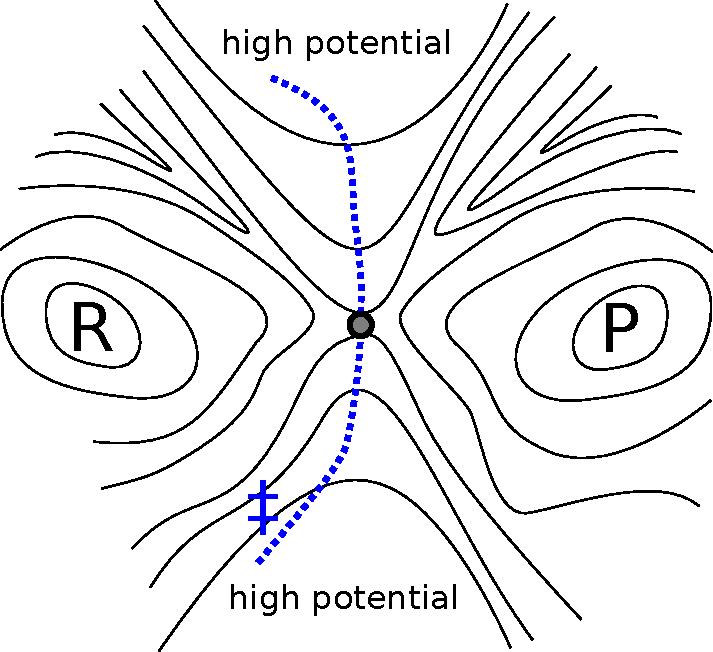
\includegraphics[width=0.5\linewidth]{transition-state}
    \parbox{0.85\linewidth}{
\caption{The transition state, $\ts$.
Representing a bottlenck region through wich all reactive trajectories (going from reactants, R, to products, P) must go.
The grey circle is a \sap{1}.
}
\label{fig:transition-state}
    }
\end{center}
\end{figure}

When dividing the phase space (position and momentum) into two areas, reactants (R) and products (P), a hypersurface separating the two emerges.
This hypersurface is referred to as the transition state ($\ts$)\footnote{The double dagger, $\ts$, is a conventional symbol for the transition state} and represents a bottleneck region with regards to the free energy, which each reactive trajectory crosses on its way from R to P.
Commonly, momentum is disregarded in the definition of the phase space, which is then $3N$ dimensional (for a system of $N$ particles), within which the $\ts$ is a $3N-1$ dimensional subspace.

\section{Reaction Rates}
Considering a canonical ensemble\footnote{The number of particles and volume is constant and there is a well defined temperature.}, the probability that a system in thermal equilibrium, i.e. described by a Boltzmann distribution, is in a given state $S$ is dependant on its configurational integral~\footnote{The continuous classical analogue to the discrete partition function.},
\beq{configurational-integral}
Z_S = \int_S e^{-E(\vR) / \kB T}d\vR
\eeq

For a hyperplanar, $\ts$, the reaction rate, $k_\text{TST}$, is defined as the probability of being in the $\ts$ subspace of $\text{R}$,
\beq{ts-probability-partition-simple}
P_\ts = \frac{Z_\ts}{Z_\text{R}},
\eeq
thermally averaged over R, with velocity away from R,
\beq{tst-rate-initial}
k_\text{TST} = \frac{1}{2}|\vect{v}_\perp| P_\ts,
\eeq
where $\vect{v}_\perp$ is the velocity component perpendicular to the $\ts$ and the factor $1/2$ comes from the fact that only half of the trajectories will be moving away from R.
Due to the different dimensionality of the $\ts$ and R, $P_\ts$ is not strictly a probability as it has the unit $\unit{m^{-1}}$ but looking at it as such aids general understanding of the rate's definition.

The velocity at each point $\vR$ can be taken from a Maxwell distribution,
\beq{tst-maxwell-velocity}
\langle |\vect{v}| \rangle = \sqrt{\frac{2kT}{\pi \mu}},
\eeq
where $\mu$ is the effective mass of the transition.
The rate then becomes
\beq{tst-rate-full}
k_\text{TST} = \sqrt{\frac{kT}{2\pi m}} \frac{Z_\ts}{Z_\text{R}}.
\eeq

\subsection{Optimisation of the Rate}
Choosing a good $\ts$ is essential for the accuracy of TST.
A trajectory that crosses the $\ts$ more than once will result in a reaction rate that is higher than the exact rate.
Either it ended again in R or crossed the $\ts$ multiple times on its way to P.
Thus the $\ts$ can act as a variational parameter for the TST rate,~\cite{vtst-1938, vtst-review-1984, vtst-2005}
\beq{tst-variational-rate}
k_\text{TST} \ge k_\text{exact}.
\eeq

%Some efforts have been put into searching for optimal $\ts$s by maximising the free energy of a hyperplane~\cite{ts-opt-2001} but such methods require costly free energy calculations.

Should optimising the $\ts$ be infeasible or insufficient, a different approach can be taken to bring $k_\text{TST}$ closer to the exact rate by estimating the error and correcting for it with a multiplication factor $\kappa_\text{D} \in (0, 1]$,
\beq{tst-dynamical-corrections}
k_\text{exact} = \kappa_\text{D} \text{ } k_\text{TST}.
\eeq
By starting dynamical trajectories from the $\ts$, which must still be reasonably good, and counting the recrossings while tracking which basin the trajectories end in, a ratio between reactive trajectories and non-reactive ones can be calculated~\cite{dynamical-corrections-keck-1962},
\beq{tst-dynamical-factor}
\kappa_\text{D} = \lim_{n \rightarrow \infty} \frac{n_\text{react.}}{n},
\eeq
where $n$ is the total amount of trajectories, started from $\vR \in \ts$, and $n_\text{react.}$ is the number of trajectories that end in P.
More recent schemes (see for example~\cite{vtst-2005, dynamical-corrections-chandler-1977, dynamical-corrections-bennett-1977}) work in the same spirit, albeit slightly more rigorous.
The scheme presented in \fref{eq:tst-dynamical-factor}, nevertheless, captures the essence of dynamical corrections.
